



Un langage tr\`es connu de mod\'elisation alg\'ebrique en optimisation est AMPL, {\co {\it A Mathematical Programming Language},
 voir le livre \cite{761822}}. D\'evelopp\'e par Fourer, Gay et 
Kernighan, il a \'et\'e conçu pour r\'esoudre des probl\`emes complexes de grande dimension. {\co On peut retrouver une liste de solveurs
sur le site \url{http://en.wikipedia.org/wiki/Optimization_\%28mathematics\%29}. Comme exemple les plus connus 
de solveurs externes, on peut citer MINOS, IPOPT, 
SNOPT, KNITRO.} Une des particularit\'es du langage AMPL est qu'il a une syntaxe tr\`es proche des
expressions math\'ematiques en optimisation. 
AMPL peut fournir $\nabla f$ et $\nabla^2 f$ mais pas les ordres sup\'erieurs. Il n'est donc pour l'instant pas possible de l'utiliser 
pour les directions plus complexes.



% Malheureusement, aucun outil de DA n'est capable de traiter cette syntaxe.

D'autre part, la librairie CUTEr, {\it A Constrained and Unconstrained Testing Environment, revisited},
fait partie des librairies les plus r\'eput\'ees pour tester des algorithmes d'optimisation.
 Elle fournit une collection de probl\`emes et fonctionne sur un grand nombre de plate-formes. 
Les probl\`emes tests sont \'ecrits en SIF  {\it Standard Input Format}.
Malheureusement, même si ce code peut-être transform\'e en Fortran, il est difficilement exploitable par les outils
de diff\'erentiation automatique qui ne g\`erent pas le code SIF.
En revanche, il existe une librairie qui est un sous-ensemble de CUTEr, \'ecrite en Fortan : celle de Mor\'e, Garbow et Hillstrom (MGH) \cite{355936} 
et qui est exploitable par les outils de DA.
 Dans le choix de l'outil de diff\'erentiation automatique, {\it Tapenade} nous est apparu comme le plus ad\'equat car il marche
par transformation de code en mode inverse et direct. De plus, il traite et retourne un code en Fortran que l'on peut de nouveau diff\'erentier.
 Th\'eoriquement, il est possible d'obtenir n'importe quel ordre de d\'erivation mais nous verrons les limitations de cet outil. N\'eanmoins, 
 cet outil a d\'ej\`a fait ses preuves dans certains milieux, {\co par exemple pour mod\'eliser la circulation oc\'eanique, \cite{diffautoopa}.}

Une fois que l'impl\'ementation des d\'eriv\'ees sera faite, le but est de v\'erifier la convergence des algorithmes
 et de comparer les coûts de calculs des m\'ethodes.
La libraire de MGH\footnote{disponible sur \url{http://www.netlib.org/uncon/data/}}, permettra de traiter un large \'eventail de cas possibles et \'evaluera la fiabilit\'e et la robustesse des algorithmes.




\section{Les outils de diff\'erentiation automatique}
Il existe plusieurs outils de diff\'erentiation automatique, d'apr\`es le site sp\'ecialis\'e tr\`es connu en DA :
 autodiff\footnote{\url{http://www.autodiff.org/}}, consulter le tableau \ref{tab:outils}. Les outils qui atteignent un ordre sup\'erieur \`a deux de d\'erivation 
utilisent g\'en\'eralement le mode direct. On observe que la plupart des langages trait\'es sont
C/C++, Fortran et Matlab.


\begin{table}[H]
	\begin{center}
{
\scriptsize
%\footnotesize
%\small
\begin{tabular}{ | l | c | r | c | c | c | } \hline

           &         & Transformation            & Mode   & Mode      & Ordre  \\
  Logiciel & Langage & de code (t)               & direct &  inverse  &        \\
           &         & surcharge (s)             &        &           &        \\

\hline
 ADC &  C/C++ &  s  & 1 & 0 & 2 \\
 ADF  & Fortran77, 95 &  s  & 1 & 0 & 2 \\
 ADG  & Fortran77 & s  & 0 & 1 & $>$2  \\
 ADIC  & C/C++ & t  & 1 & 0 & 2 \\
 ADIFOR  & Fortran77 & t  & 1 & 0 &  2\\
 ADiMat  & MATLAB &  t & 1 & 0 & 2 \\
 ADMAT / ADMIT  & MATLAB & s  & 1 & 1 & 2\\
 ADOL-C  & C/C++ & s  & 1 & 1 & $>$2 \\
 ADOL-F  & Fortran95 & s  & 1 & 1 & $>$2\\
%  APMonitor  & Interpreted & s  & 1 & 0 &  \\
 AUTO\_DERIV  & Fortran77, 95 & s  & 1 & 0 & 2\\
 COSY INFINITY  & Fortran77, 95,C/C++ & s  & 1 & 0 &$>$2 \\
 CppAD  & C/C++ & s  & 1 & 1 & $>$2 \\
 FAD  & Haskell & s  & 1 & 0 & $>$2  \\
 FADBAD/TADIFF  & C/C++ & s  & 1 & 1 & $>$2 \\
 FFADLib  & C/C++ & s  & 1 & 0 & 2 \\
 GRESS  & Fortran77 & t  & 1 & 1 & 1  \\
 HSL\_AD02  & Fortran95 & s  & 1 & 1 & $>$2 \\
 INTLAB  & MATLAB & s  & 1 & 0 & 2 \\
 NAGWare Fortran 95   & Fortran77, 95 & t  & 1 & 0 & $>$2 \\
 OpenAD  & C/C++,Fortran77, 95 &  t  & 1 & 1 & 2  \\
 PCOMP  & Fortran77 & t  & 1 & 1 & 2 \\
 pyadolc  & python & s  & 1 & 1 & 2 \\
 pycppad  & Interpreted,python & s  & 1 & 1 & $>$2\\
 Rapsodia  & C/C++,Fortran95 & s  & 1 & 0 &  $>$2\\
 Sacado  & C/C++ & s  & 1 & 1 & 1 \\
 TAF  & Fortran77, 95 & t  & 1 & 1 & 2 \\
 TAMC  & Fortran77 & t  & 1 & 0 & 1 \\
 TAPENADE  & C/C++,Fortran77, 95 & t  & 1 & 1 & $>$2 \\
%  TaylUR  & Fortran95 &
 TOMLAB /TomSym  & MATLAB & t/s & 1 & 1 & 2\\
\hline


\end{tabular}
}
	\end{center}
	\caption{Plusieurs outils de DA}
	\label{tab:outils}
\end{table}





% Etant donn\'e que nous voulons adapter un outil sous scilab, il est plus facile de lier une librairie 
% au langage Fortran. Nous avons fait le choix de {\it Tapenade} car il traite du code Fortran et permet de produire 
% un code diff\'erenti\'e qui pourra de nouveau être trait\'e. Ainsi, n'importe quel ordre peut être atteint. \\



\section{Un outil de DA: {\it Tapenade}}
\label{sec:tapenade}

%     \subsection{Historique}

{\it Tapenade}\footnote{disponible sur \url{http://www-sop.inria.fr/tropics/}} est un outil de diff\'erentiation automatique qui a commenc\'e \`a être d\'evelopp\'e en 1999
par une \'equipe du projet Tropics \`a l'INRIA. 
% {\it Tapenade} est l'acronyme pour Transformations et Outils Informatiques Pour le Calcul
% Scientifique.
 Il utilise la transformation de code. L'avantage, c'est que l'on va pouvoir diff\'erentier plusieurs fois
puisque le code diff\'erenti\'e est vu comme une routine classique.

    \subsection{Comment utiliser la DA pour les d\'eriv\'ees d'un point de vue th\'eorique}

Ce que l'on cherche, c'est obtenir les d\'eriv\'ees successives du code Fortran de mani\`ere efficace pour 
une dimension assez grande $n=1000$.

$$F=\nabla f \in \mathbb{R}^n \rightarrow \mathbb{R}^n$$
Nous voulons l'expression $\nabla^2 f\cdot v$. Pour calculer par diff\'erentiation automatique, nous allons utiliser l'astuce 
suivante :
$$\nabla_x(\nabla_x f(x) \cdot d)) = \nabla_{xx}^2f(x) \cdot d$$ O\`u $d$ repr\'esente la direction obtenue.
Au lieu de calculer la hessienne, nous allons appliquer le mode direct sur le calcul du gradient par un vecteur.
Regardons sur un exemple : 
$$f(x)=x_1^3x_2^2-10x_1x_2-x_2^3$$
$$\nabla_x f(x)=F(x)=\left( \begin{array}{cc}3x_1^2x_3^2-10x_2 & 2x_1^3x_2-10x_1-3x_2^2\end{array} \right)$$
$$\nabla_{xx}^2f(x)=\left( \begin{array}{cc}
6x_1x_2^2 & 6x_1^2x_2-10 \\
6x_1^2x_2-10 &  2x_1^3-6x_2 \\
\end{array} \right)$$

$$d = \left( \begin{array}{c} 1 \\2 \\ \end{array} \right)$$

$$\nabla_xf(x).d=3x_1^2x_2^2-10x_2+4x_1^3x_2-20x_1-6x_2^2$$
$$\nabla_x(\nabla_x f(x) \cdot d))=
\left( \begin{array}{cc} 6x_1x_2^2+12x_1^2x_2-20 & 6x_1^2x_2-10+4x_1^3-12x_2 \end{array} \right) $$ 

$$\nabla_{xx}^2f(x).d =
 \left( \begin{array}{c} 6x_1x_2^2+12x_1^2x_2-20\\6x_1^2x_2-10+4x_1^3-12x_2 \\ \end{array} \right) $$
%
%
Puisque la matrice hessienne est sym\'etrique, on remarque bien que 
$$\left( \nabla_{xx}^2f(x).d \right)^T = \nabla_x(\nabla_xf(x).d))$$
%
%
En mode inverse :
$$\psi(t)=F(x+t \cdot d)=F(g(t))$$
$g(t)=x+t \cdot d$ o\`u $d$ repr\'esente la direction
$$\psi'(t)=\nabla F(x+t \cdot d)d$$
$$\psi'(0)=\nabla F(x)d$$
%
Ainsi, pour obtenir $\nabla^2 f(x)\cdot v$, nous appliquons le mode direct apr\`es le mode inverse.
Le fait d'appliquer ces deux modes, l'un apr\`es l'autre nous donnent le bon r\'esultat uniquement parce qu'\`a la base
nous utilisons une fonction scalaire et que la matrice hessienne est sym\'etrique. Dans le cas contraire, si la $i$\`eme ligne de $\nabla^2 f$ 
ne correspondrait pas \`a sa $i$\`eme colonne et nous ne pourrions pas utiliser ce proc\'ed\'e. \`A partir de l\`a, nous pouvons r\'eappliquer plusieurs fois 
le mode direct pour atteindre $\nabla (\nabla f \cdot d)\cdot d$.



    %\subsection{La librairie MGH}
    \subsection{Utilisation de {\it Tapenade}}

L'outil peut s'utiliser soit en local, soit en ligne grâce \`a un serveur. Son utilisation s'effectue en plusieurs \'etapes.
D'abord, il faut fournir le code en Fortran qui contient le code \`a diff\'erentier sous la forme d'un fichier. Ensuite,
il faut d\'efinir la routine que l'on souhaite diff\'erentier et les variables d'entr\'ees par rapport \`a laquelle la diff\'erentiation doit
être faite et les variables de sortie d\'ependantes. Enfin, il faut choisir le mode : tangent, inverse ou multi-directionnel.
Supposons que la variable de sortie est $Y \in \mathbb{R}^n$, d\'ependante de $X \in \mathbb{R}^m$. En fait, nous avons $Y=f(X)$ avec
$f:\mathbb{R}^m\rightarrow\mathbb{R}^n$. Notons $J:=\nabla f \in \mathbb{R}^n\times\mathbb{R}^m$ la matrice jacobienne de $f$.
La routine contient donc les arguments $Y$; une variable r\'esultat et $X$ la variable d'entr\'ee.


\paragraph{Mode direct} \hfill \\
Comme expliqu\'e dans le paragraphe \ref{chap2:tangent}, en plus de sp\'ecifier la variable d'entr\'ee $X$,
 nous allons aussi sp\'ecifier une variation $dX$ sur
 laquelle la jacobienne va s'appliquer.\\


$\left( 
\begin{array}{c} 
\dot{y_1} \\
\dot{y_2} \\
\vdots \\
\dot{y_m}

\end{array}
\right)
=dY = J(X) \times dX =
\underbrace{
\left( 
\begin{array}{ccccc} 
\frac{\partial y_1}{\partial x_1} & \frac{\partial y_1}{\partial x_2} &
 \frac{\partial y_1}{\partial x_3} & \cdots & \frac{\partial y_1}{\partial x_m} \\
\frac{\partial y_2}{\partial x_1} & \frac{\partial y_2}{\partial x_2} &
 \frac{\partial y_2}{\partial x_3} & \cdots & \frac{\partial y_2}{\partial x_m} \\
\vdots & \vdots & \vdots & \ddots & \vdots \\
\frac{\partial y_n}{\partial x_1} & \frac{\partial y_n}{\partial x_2} &
 \frac{\partial y_n}{\partial x_3} & \cdots & \frac{\partial y_n}{\partial x_m} \\
\end{array}
\right)}_{\text{Jacobienne en }X}
 \times
\left( 
\begin{array}{c} 
\Tilde{x_1} \\
\Tilde{x_2} \\
\vdots \\
\Tilde{x_m}
\end{array}
\right)
 $ \\
%
Par exemple, si $dX$ est initialis\'ee \`a $e_1$, nous aurons la premi\`ere colonne de la Jacobienne et si $Y$ est un scalaire 
nous aurons la premi\`ere composante de son gradient. Deux nouvelles variables vont être ajout\'ees. De la routine\\
\verb!SUBROUTINE FONCTION(X,Y)!\\
le logiciel g\'en\`ere :\\
\verb!SUBROUTINE FONCTION_D(X, Xd, Y, Yd)!\\
o\`u {\tt Y}, {\tt Yd} sont les variables de sortie et {\tt X}, {\tt Xd} les variables d'entr\'ee. On a donc
{\tt Y=}$F${\tt (X)} et {\tt Yd=}$\nabla F${\tt (X).Xd}


Le mode multidirectionnel revient \`a appliquer \`a plusieurs vecteurs {\tt Xd}, en fait {\tt Xd} est une matrice. %En utilisant le mode directe sur m $(dX)_i=I$ 


\paragraph{Mode inverse} \hfill \\
De même, un vecteur doit être sp\'ecifi\'e en mode inverse mais comme le calcul se fait \`a rebours, l'op\'eration 
est invers\'ee.




$\left( 
\begin{array}{c} 
\bar{x_1} \\
\bar{x_2} \\
\vdots \\
\bar{x_m}

\end{array}
\right)
=dX = \underbrace{J^*(X)}_{J(X)^T} \times dY = 
\underbrace{
\left(
\begin{array}{ccccc} 
\frac{\partial y_1}{\partial x_1} & \frac{\partial y_2}{\partial x_1} &
 \frac{\partial y_3}{\partial x_1} & \cdots & \frac{\partial y_n}{\partial x_1} \\
\frac{\partial y_1}{\partial x_2} & \frac{\partial y_2}{\partial x_2} &
 \frac{\partial y_3}{\partial x_2} & \cdots & \frac{\partial y_n}{\partial x_2} \\
\vdots & \vdots & \vdots & \ddots & \vdots \\
\frac{\partial y_1}{\partial x_m} & \frac{\partial y_2}{\partial x_m} &
 \frac{\partial y_3}{\partial x_m} & \cdots & \frac{\partial y_n}{\partial x_m} \\
\end{array}
\right)}_{\text{Transpos\'ee de la jacobienne en }X}
 \times
\left( 
\begin{array}{c} 
\bar{y_1} \\
\bar{y_2} \\
\vdots \\
\bar{y_m}

\end{array}
\right)
 $ \\ 
En reprenant le même exemple de 
\verb!SUBROUTINE FONCTION(X,Y)!\\
{\it Tapenade} g\'en\`ere :\\
\verb!SUBROUTINE FONCTION_B(X, Xb, Y, Yb)!\\
cette fois-ci {\tt Y} et {\tt \underline{Xb}}$:=dX$ sont les variables de sortie et {\tt X}, {\tt\underline{Yb}}$:=dY$ les variables d'entr\'ee. 
Si nous appliquons sur $dY=e_i$ nous obtiendrons la $i$\`eme ligne de la jacobienne.
Le calcul correspond \`a {\tt Xb=}$\nabla F(${\tt X}$)^T${\tt Yb}





\paragraph{D\'eriv\'ees sup\'erieures} 
Pour les ordres sup\'erieurs, nous allons r\'eappliquer le même proc\'ed\'e sur les fonctions obtenues. Par exemple appliquer le mode direct sur 
le mode inverse, c'est-\`a-dire sur la routine \verb!SUBROUTINE FONCTION_B(X, Xb, Y, Yb)!\\
En sp\'ecifiant de diff\'erentier {\tt Xb} par rapport \`a {\tt x} : \\
\verb! SUBROUTINE FONCTION_B_D(X, Xd, Xb, Xbd, Y, Yb)!\\
variables d'entr\'ee \verb!X Xd Xb Yb!\\
variables de sortie \verb!Xbd, Y!\\
{\tt Xbd}=$\nabla(\nabla F${\tt (X)}$\cdot${\tt Yb}$)^T)\cdot${\tt Xd}\\



Malheureusement, le logiciel {\it Tapenade} n'a pas \'et\'e conçu pour obtenir des d\'eriv\'ees sup\'erieures \`a deux avec le mode inverse. D'autre
part le mode inverse sur inverse n'existe pas (il serait trop compliqu\'e \`a g\'erer).
\`A l'aide d'un Makefile, j'ai g\'en\'er\'e l'ensemble des d\'eriv\'ees dont j'avais besoin. Pour chaque fonction, 
plusieurs fichiers sont g\'en\'er\'es : un pour chaque op\'eration que l'on souhaite. Pour atteindre les d\'eriv\'ees
d'ordre sup\'erieur, les fichiers g\'en\'er\'es sont redonn\'es \`a l'outil pour être de nouveau diff\'erenti\'es.



% Voir \ref{annexe:Ctap}.

% \label{annexe:Ctap}
% Lorsque l'on fait du mode inverse, une pile est cr\'e\'ee afin de stocker les variables. Ensuite,
% si on applique le mode direct, on va devoir g\'erer une double pile.
% Ainsi, au lieu d'avoir {\tt PUSHREAL8(u)}, nous avons {\tt PUSHREAL8\_D(u, ud)}.
% Pour chaque nouvelle d\'eriv\'ee, une nouvelle pile va \^etre additionn\'ee. Cependant, seules
% {\tt PUSHREAL8\_D} et {\tt PUSHREAL8\_D} ont \'et\'e cr\'eees. J'ai dû \'ecrire 
% {\tt PUSHREAL8\_D\_D} et {\tt PUSHREAL8\_D\_DV}. Malheureusement, cela ne suffit pas 
% et dans le code g\'en\'er\'e, certaines routines ne sont pas les bonnes {\tt PUSHREAL8\_D} au lieu
% de {\tt PUSHREAL8\_D\_DV}.
% 






    \subsection{Tests sur la librairie de Mor\'e, Garbow, Hillstrom}




% 
% Pour \'evaluer les temps de calcul de ces op\'erations critiques, j'ai utilis\'e les fonctions trigonom\'etrique et 
% chebyquad.
% 
% 
% \subsection{Matrices creuses}
\'Etant donn\'e que nous voulons faire des tests de calcul sur des fonctions types, il est pertinent
d'\'etudier le comportement des fonctions et notamment si la matrice hessienne est creuse.
La figure \ref{fig:trigo} indique par des points les \'el\'ements non nuls de la matrice hessienne
pour la fonction trigonom\'etrique.
On n'exploite pas le fait que la matrice soit creuse mais les coûts de calculs seront probablement
diminu\'es quand même car les op\'erations seront faites sur des z\'eros.



% \begin{figure}
% \caption{Matrice hessienne de la fonction disc\`ete \`a valeurs finies (28)}
% \center
% 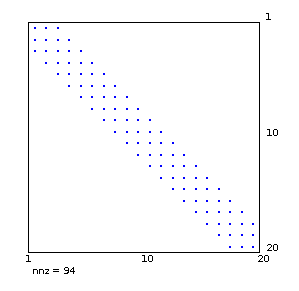
\includegraphics[scale=0.7]{figures/bound.png}
% \label{fig:bound}
% \end{figure}
% 
Nous allons pr\'esenter trois exemples de fonction appartenant \`a la librairie; la fonction bien connue en optimisation Rosenbrock, g\'en\'eralis\'ee \`a dimension variable, 
une fonction trigonom\'etrique et une fonction utilisant les polynômes de Chebychev.
% 
% 
% 
% Comme les polynômes sont de plus en plus compliqu\'es \`a calculer quand la dimension augmente, le coût de $f$
% ne va pas être lin\'eaire par rapport \`a $n$.



\paragraph{Fonction trigonom\'etrique}
\begin{align*}
% \begin{equation}
n \text{ variable, } m=n \\
f_i(x)=n-\sum_{j=1}^{n}cos(x_j)+i(1-cos(x_i))-sin(x_i) \\
x_0= [1/n, \cdots , 1/n] \\
min_x f(x) = 0
% \end{equation}
\end{align*}

% \begin{figure}
% \caption{Matrice hessienne de la fonction trigonom\'etrique}
% \center
% 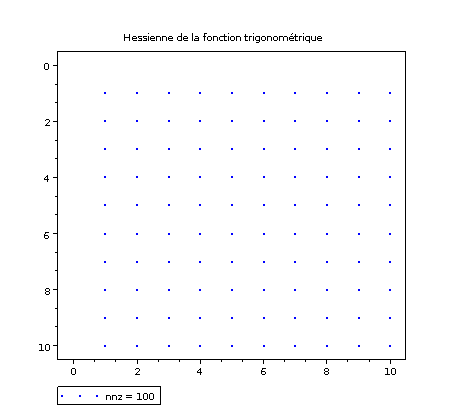
\includegraphics[scale=0.4]{figures/trigo.png}
% \label{fig:trigo}
% \end{figure}


\begin{figure}
\caption{Matrice hessienne de taille 10 par 10 de la fonction trigonom\'etrique, les points bleus repr\'esentent les \'el\'ements non nuls de la
matrice.}

\begin{center}
\fbox{
\begin{minipage}[c]{0.36\textwidth}
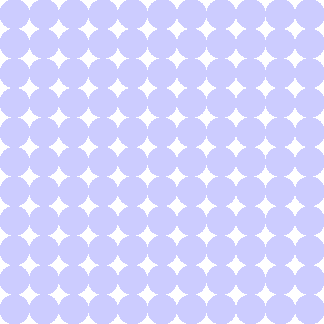
\includegraphics[scale=1]{figures/figure_16}
\end{minipage}
}
\end{center}
\label{fig:trigo}
\end{figure}






La matrice hessienne de la fonction trigonom\'etrique est une matrice pleine \ref{fig:trigo}, cette fonction pourra nous servir 
de r\'ef\'erence car les calculs sont relativement simples.



% \subsection{Fonction Rosenbrock \'etendue}
\paragraph{La fonction Rosenbrock \'etendue}

\begin{align*}
n\text{ variable mais pair } m=2 \\
f_{2i-1}(x)=10(x_{2i}-x^2_{i-1})\\
f_{2i}(x)=1-x_{2i-1}\\
x_0= (\xi_i) \text{ o\`u } \xi_{2i-1}= -1.2  \text{ et } \xi_{2i}=1 \\
min_x f(x) = 0 \text{ en } [1,\cdots ,1]
\end{align*}

Chaque composante de la fonction n'est d\'ependante que de deux variables, c'est pourquoi la matrice hessienne est creuse.

\begin{figure}
\caption{Matrice hessienne de la fonction de Rosenbrock \'etendue}
\begin{center}
\fbox{
\begin{minipage}[c]{0.36\textwidth}
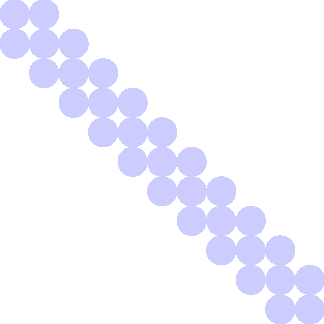
\includegraphics[scale=1]{figures/figure_17}
\end{minipage}
}
\end{center}
\label{fig:rosenbrock}
\end{figure}



% \begin{figure}
% \caption{Newton - La recherche lin\'eaire restreint \`a fournir des it\'er\'es dont la valeur de l'objectif est 
% toujours d\'ecroissante tandis que sans recherche, on s'\'eloigne pour converger plus vite.}
% \begin{center}
% \fbox{
% \begin{minipage}[c]{0.6\textwidth}
% 
% \end{minipage}
% }
% \end{center}
% \label{fig:Newton}
% \end{figure}




La fonction a \'et\'e propos\'ee par Rosenbrock en 1960 afin de comparer des algorithmes de descente. Dans 
le cas avec $n=2$, la fonction forme un sillon \'etroit, ce qui oblige les m\'ethodes de descente \`a suivre une courbe. 
L'agorithme du gradient par exemple est tr\`es m\'ediocre car il "rebondit" sur chaque parois sans avancer vraiment {\co \ref{fig:grarosenbrock}.
La figure de gauche montre les lignes de niveau de la fonction et les droites en bleues correnpondent aux it\'er\'es de l'algorithme du gradient.
L'it\'er\'e initial est \`a gauche et la solution \`a droite. Au milieu, le "saut" a \'et\'e trouv\'e par une recherche lin\'eaire avanc\'ee. La figure de droite
est un zoom de l'algorithme, nous pouvons observer la difficult\'e \`a trouver une direction qui permet d'avancer plus efficacement.}
En ce qui concerne la m\'ethode de Newton, augmenter la dimension de la fonction n'influencera pas le nombre d'it\'erations
car le probl\`eme pourra être vu comme $\frac{n}{2}$ probl\`emes de Rosenbrock qui s'effectuent parall\`element.




\begin{figure}[h]
\caption{Alogrithme du gradient sur Rosenbrock : 19436 it\'erations}
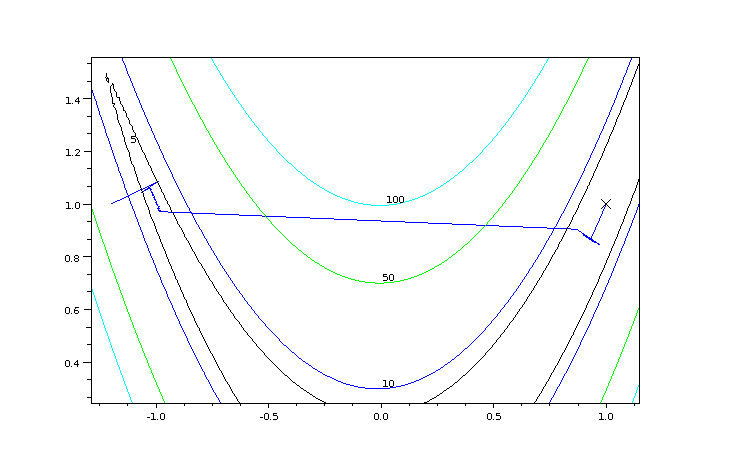
\includegraphics[scale=0.3]{figures/gradient.png}
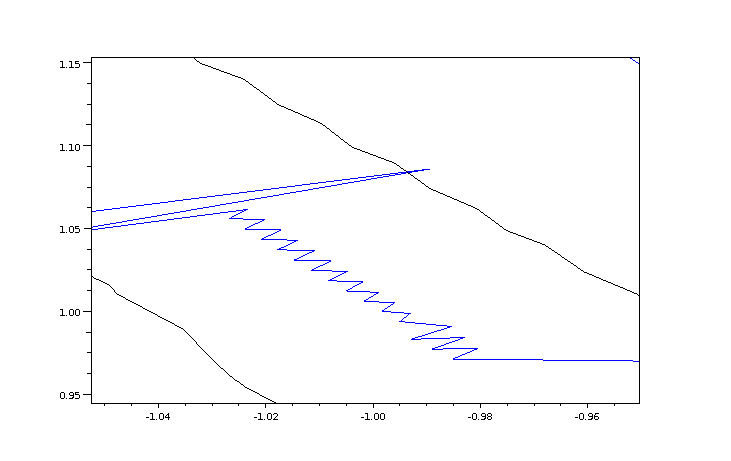
\includegraphics[scale=0.3]{figures/gradientzoom.png}
\label{fig:grarosenbrock}
\end{figure}




% \subsection{Fonction Chebyquad}
\paragraph{La fonction Chebyquad}

\begin{align*}
n \text{ variable, } m=n \\
f_i(x)=\frac{1}{n}\sum_{j=1}^{n}T_i(x_j)-\int_0^1 \! T_i(x)dx \\
\text{O\`u }T_i\text{ est le i\`eme polynôme de Chebychev r\'eduit \`a l'intervale } [0,\ 1] \\
\int_0^1 \! T_i(x)dx= 0 \text{ pour i paire}\\
\int_0^1 \! T_i(x)dx= \frac{-1}{i^2-1} \text{ pour i impaire}\\
x_0= (\xi_j) \text{ o\`u } \xi_j=j/(n+1)\\
f=0 \text{ pour } m=n \text{,}\ 1\leq n\leq 7\ \text{ et }\ n=9\\
f=3.51687... 10^{-3}\ \text{ pour }\ n=m=8 \\
f=6.50395... 10^{-3}\ \text{ pour }\ n=m=10 \\
\end{align*}



% \begin{figure}
% \caption{Matrice hessienne de la fonction de Chebyquad}
% \center
% 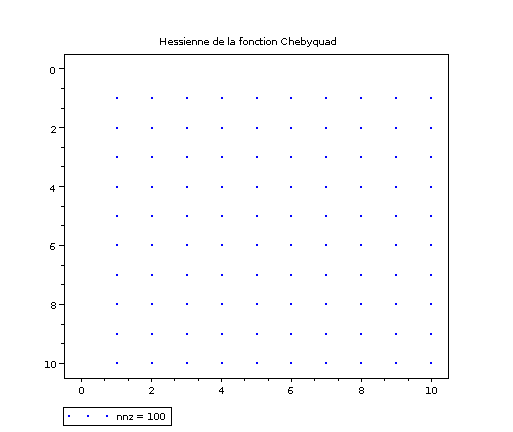
\includegraphics[scale=0.4]{figures/chebyquad.png}
% \label{fig:chebyquad}
% \end{figure}

\begin{figure}
\caption{Matrice hessienne de la fonction de Chebyquad}
\begin{center}
\fbox{
\begin{minipage}[c]{0.36\textwidth}
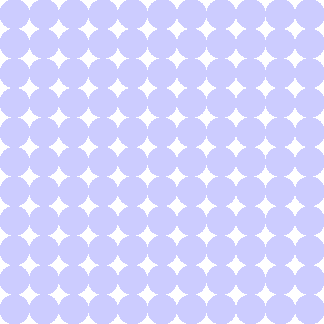
\includegraphics[scale=1]{figures/figure_16}
\end{minipage}
}
\end{center}
\label{fig:chebyquad}
\end{figure}




Ces trois fonctions ont des dimensions variables ; elle refl\`etent l'ensemble des r\'esultats qui sont \'equivalents pour les calculs des d\'eriv\'ees.
La fonction Chebyquad est plus particuli\`ere dans le sens o\`u le temps d'ex\'ecution de la fonction n'est pas proportionnel
\`a la dimension car les polynômes sont de plus en plus complexes \`a calculer en fonction de $n$. 





\paragraph{Temps de calcul du gradient fourni par la routine et du gradient recod\'e}
 Pour la fonction trigonom\'etrique, comme le montre \ref{fig:temps14},
 le calcul du gradient donn\'e par la routine de netlib n'est pas 
efficace. Ceci s'explique par le fait que pour l'obtenir, on utilise la relation $$ \nabla f(x)=F(x)^T\nabla F(x)$$ en notant que 
$$f(x)= \frac{1}{2}\sum_{i=1}^{m}F_i(x)^2$$
Le calcul de la Jacobienne $\nabla F(x)$ de taille $n$ par $m$ impose beaucoup de calculs qui peuvent être \'evit\'es.
En recodant le gradient de la fonction, les multiplications sur les lignes sont factorisables, et en \'evitant le calcul de la 
jacobienne, on am\'eliore nettement l'ex\'ecution. {\co Pour une dimension relativement grande, le temps de calcul du gradient fourni prend plusieurs seconde 
alors que celui de la fonction recod\'e de mani\`ere optimis\'e est instantan\'e.}




\begin{figure}
\caption{Temps d'\'evaluation du gradient en modifiant la taille
de $x$ et celui du gradient recod\'e}
\center
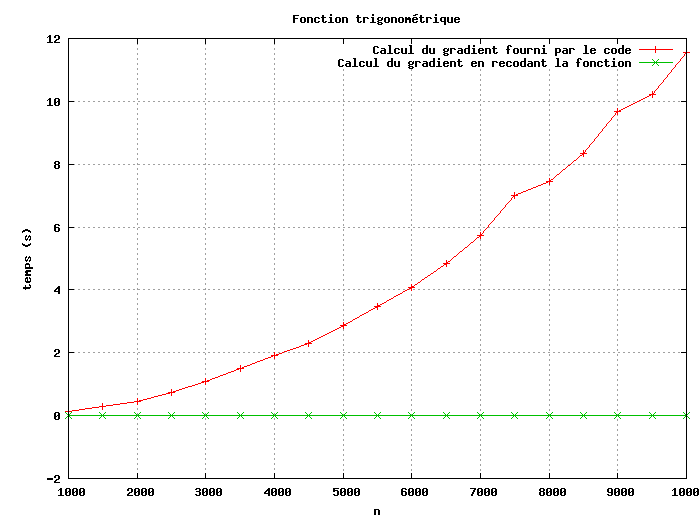
\includegraphics[scale=0.4]{figures/temps14.png}
\label{fig:temps14}
\end{figure}


% \begin{figure}
% \caption{Gradient de la fonction trigonom\'etrique dont le code \`a \'et\'e am\'elior\'e comparativement \`a celui d'origine}
% \center
% 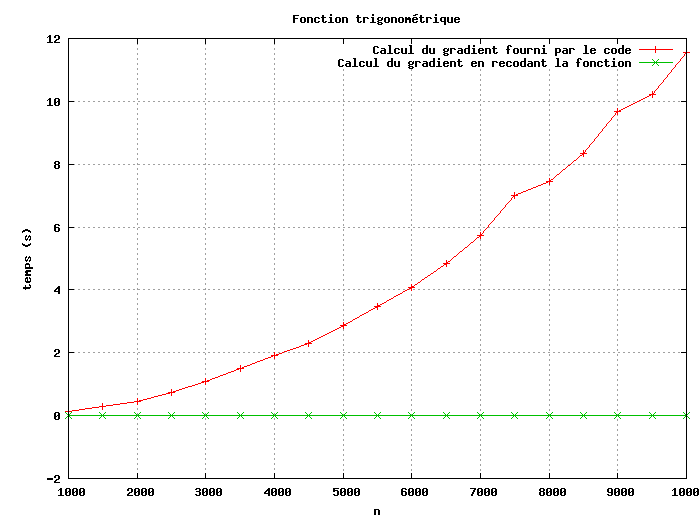
\includegraphics[scale=0.4]{figures/temps14.png}
% \label{fig:temps14}
% \end{figure}




% Avec le code g\'en\'er\'e par tapenade :
% Tableau pour calculer $f(x)$, $\nabla f(x)$,$\nabla^2 f(x)$, $\nabla f(x).v$, $\nabla^2 f(x).uv$



 \paragraph{Comparaison entre l'\'evaluation de la fonction et le mode inverse}

Afin de pouvoir comparer les temps d'ex\'ecution de la fonction et du mode inverse, les appels sont faits
plusieurs fois dans une boucle de mille it\'erations. En effet, même pour une dimension de $n=10000$,
 le temps pour \'evaluer la fonction est inf\'erieur au pas d'horloge unitaire de $4$ms. On remarque sur la
 figure \ref{fig:temps2} que l'obtention du gradient par le mode
inverse est clairement proportionnel au coût de la fonction avec un facteur de proportionnalit\'e d'environ
deux; pour rappel, la borne th\'eorique est de quatre. Le mode inverse est nettement plus performant qu'une implantation na\"ive.


\begin{figure}
\caption{Temps de calcul de la fonction et du gradient en mode direct par {\it Tapenade} dans une boucle de mille it\'erations, fonction trigonom\'etrique}
\center
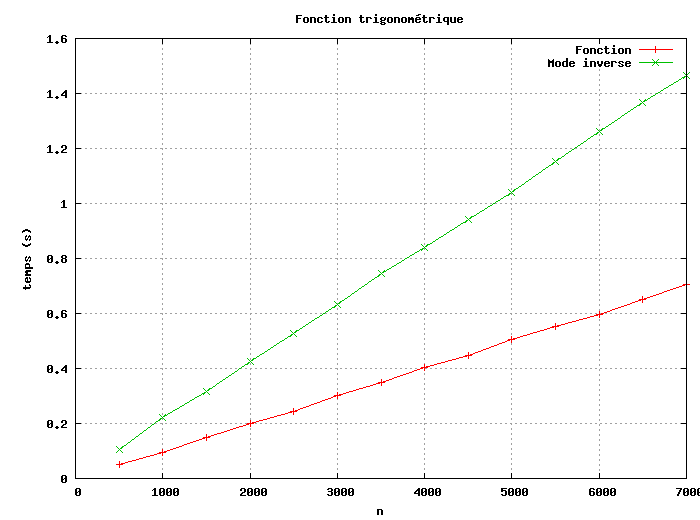
\includegraphics[scale=0.4]{figures/temps2.png}
\label{fig:temps2}
\end{figure}


% La figure \ref{fig:temps6} montre que l'\'evaluation de la fonction Chebyquad n'est pas proportionnelle \`a la dimension; il ne s'agit pas d'une droite.
% En revanche, le gradient ressemble \`a un facteur pr\`es \`a celle de l'\'evaluation. On peut observer que $\#(\nabla f)\simeq 3.5 \#(f)$.
% 
% 
% \begin{figure}
% \caption{Fonction chebyquad, mode inverse vs temps fonction, l'\'evaluation n'est pas proportionnelle \`a la dimension, par contre le gradient 
% ressemble \`a un facteur pr\`es \`a $f$}
% \center
% 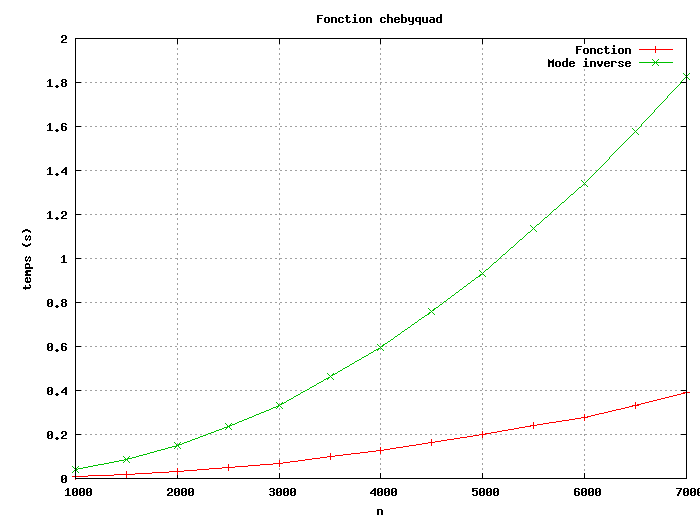
\includegraphics[scale=0.4]{figures/temps6.png}
% \label{fig:temps6}
% \end{figure}



\paragraph{Le mode multi-directionnel}
Le mode multi-directionnel correspond au mode direct appliqu\'e \`a chacune des composantes;
il \'equivaut \`a effectuer $\nabla f(x).(e_i)$ pour chaque $1\leq i\leq n$.
Dans la figure \ref{fig:temps1}, nous pouvons voir que le temps en mode multi-directionnel est
 environ le même que pour calculer le gradient par diff\'erences finies. Le mode multi-directionnel
n'est pas avantageux puisqu'il effectue le mode tangent $n$ fois. {\co La figure \ref{fig:temps4}
permet de comparer le mode multi-directionnel et le mode inverse; pour une dimension assez grande,
le temps de calcul pour le mode multi-directionnel est insatisfaisant et il sera pr\'ef\'erable de l'\'eviter
tant que c'est possible.}

\begin{figure}
\caption{Temps de calcul - fonction trigonom\'etrique}
\center
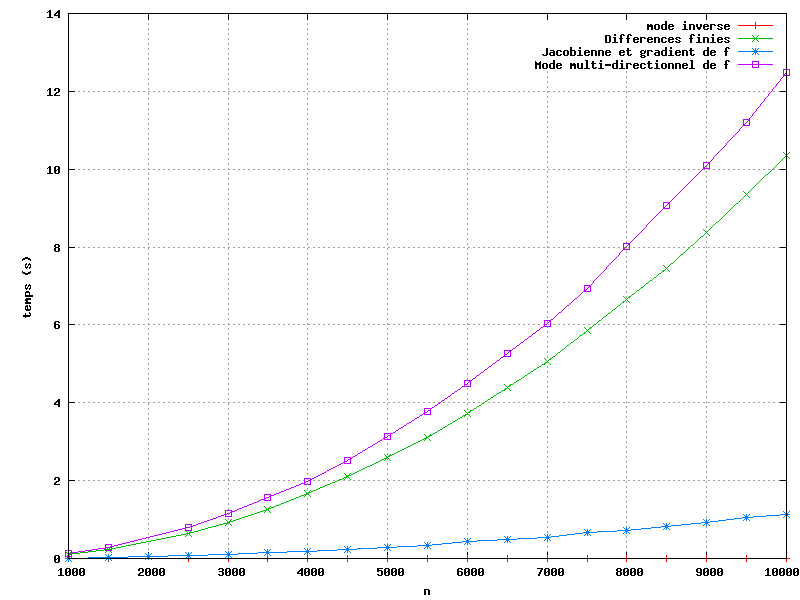
\includegraphics[scale=0.4]{figures/temps1.png}
\label{fig:temps1}
\end{figure}

\begin{figure}
\caption{Mode multi-directionnel : $\nabla f(x)$}
\center
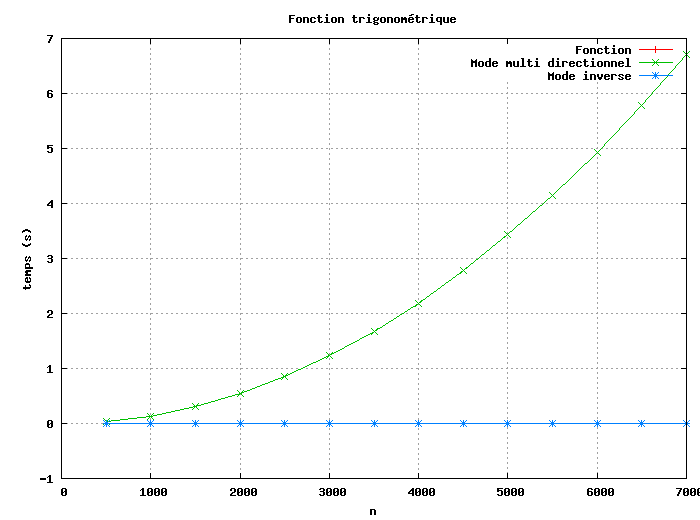
\includegraphics[scale=0.4]{figures/temps4.png}
\label{fig:temps4}
\end{figure}


\paragraph{Hessien$\times$vecteur}

Comme pour le mode inverse, le coût du hessien multipli\'e par un certain vecteur calcul\'e par mode direct sur mode inverse est proportionnel
 au coût de la foncion \ref{fig:temps3} environ 4$\times\#(f)$. {\co En effet, les trois courbes sont tr\`es proches de droites. Ainsi, nous validons
bien que la borne de complexit\'e de $\nabla^2f(x)\cdot v$ est $\mathcal{O}(\#(f))$.}


\begin{figure}
\caption{Mode tangent sur inverse (vert $\times$) sur une boucle de mille it\'erations, ce qui correspond au calcul de $\nabla^2 f(x).v$ pour un certain vecteur, le r\'esultat
est donc aussi un vecteur}
\center
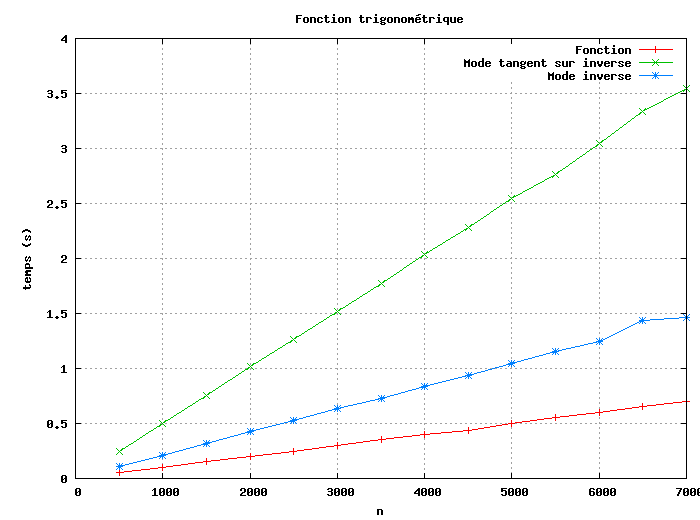
\includegraphics[scale=0.4]{figures/temps3.png}
\label{fig:temps3}
\end{figure}






\paragraph{Hessien}

Pour obtenir la matrice hessienne \ref{fig:temps16}, nous avons pas le choix d'appliquer le mode multi-directionnel. Nous observons cette 
fois ci que le coût est proportionnel \`a $n$ fois le coût de l'\'evaluation de la fonction.


\begin{figure}
\caption{Mode multi-directionnel sur inverse (vert $\times$) ce qui donne la hessienne $\nabla^2 f(x)$ pour un certain vecteur, le r\'esultat
est donc aussi un vecteur}
\center
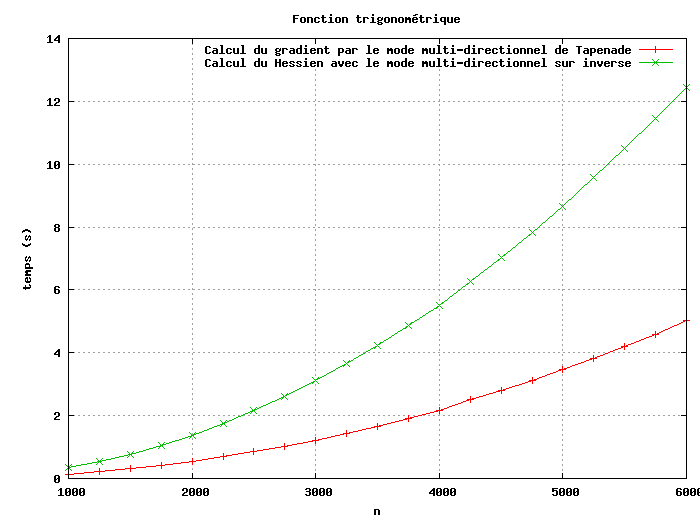
\includegraphics[scale=0.4]{figures/temps16.png}
\label{fig:temps16}
\end{figure}





\paragraph{Ordres sup\'erieurs}
Le coût des op\'erations $\nabla^3 f(x)\cdot u \cdot v$ et $\nabla^4f(x)\cdot u \cdot v \cdot w$ ne d\'ependent pas de $n$ comme le montre la figure
\ref{fig:temps17}. Toutes les courbes sont affines.

\begin{figure}
\caption{Temps des op\'erations  $\nabla^4f(x)\cdot u \cdot v \cdot w$ en vert et marron, $\nabla^3 f(x)\cdot u \cdot v$ en rouge : elles ne d\'ependent pas de $n$
et sont proportionnelles au coût de la fonction.}
\center
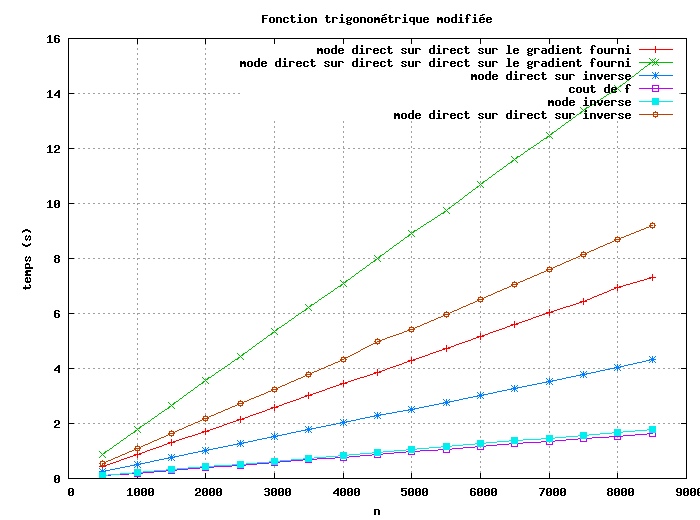
\includegraphics[scale=0.4]{figures/temps17.png}
\label{fig:temps17}
\end{figure}



    \subsection{Avantages et inconv\'enients de {\it Tapenade}}

La transformation du code est la meilleure approche pour la DA; elle donne la capacit\'e de calculer les gradients
\`a un faible coût puisqu'elle ex\'ecute de mani\`ere imp\'erative comme le programme original. De plus, il n'y a pas 
de restriction sur le style ou la taille de l'application \`a diff\'erentier. Au lieu de coder \`a la main une fonction
poss\'edant plusieurs millions de lignes, ce qui est source d'erreurs et demande un effort consid\'erable, il est plus pratique 
de le faire automatiquement. C'est un outil qui progresse encore; les performances du calcul de l'adjoint sont en cours 
d'am\'elioration.
Cependant, il ne traite que du code Fortran et C, même si th\'eoriquement, tous les langages peuvent être trait\'es. Le
sch\'ema optimal de checkpoints imbriqu\'es pour un programme quelconque reste un probl\`eme de recherche.
De plus, les boîtes noires ne peuvent \'evidemment pas être g\'er\'ees, ce qui n'est pas le cas pour la diff\'erentiation par diff\'erences
finies. Pour finir, la plus grosse difficult\'e vient du fait que le logiciel ne g\`ere pas l'ordre trois avec le mode inverse. Il a donc
fallu adapter la librairie mais malgr\'e tout, certains cas ne sont pas fiables, et donne par exemple une hessienne non sym\'etrique.




    \subsection{Difficult\'es pour les d\'eriv\'ees sup\'erieures}

La complexit\'e du stockage des variables lors de la diff\'erentiation automatique est expliqu\'ee dans le livre de Griewank
 \cite{Griewank2008EDP}. Il analyse entre autres le stockage des variables avec l'ordre des op\'erations atomiques et le 
mode inverse r\'ep\'et\'e. Bien qu'efficace, le mode inverse comporte des complications avec {\it Tapenade},
 lorsque l'on veut diff\'erentier \`a un ordre sup\'erieur.
Contrairement au mode tangent qui ne fait que rajouter des op\'erations \'el\'ementaires dans le code, le mode inverse
va faire apparaître des appels \`a des routines : {\tt PUSH} et {\tt POP}. Celles-ci vont permettre de g\'erer une pile qui 
alternativement stockera et restituera les variables tel que d\'ecrit \`a la section \ref{subsection:strategies}. Elles sont cod\'ees en C et appartiennent 
\`a une libraire ext\'erieure mais ne sont pas fournies \`a l'outil de diff\'erentiation. Leur propre code adjoint a \'et\'e cod\'e manuellement
mais seulement \`a l'ordre un par {\it Tapenade}. Pour obtenir des d\'eriv\'ees d'ordre trois, il a fallu coder leurs d\'eriv\'ees.
Lorsque l'on effectue le mode tangent sur tangent sur inverse, certaines routines correspondant aux PUSH et POP ne sont pas correct et il a fallu
les modifier de mani\`ere automatique. Malgr\'e cela, il existe de rares cas o\`u la matrice hessienne n'est pas sym\'etrique mais anti-sym\'etrique. 


{\co 
\section{Conclusion}

Ce chapitre valide les bornes de complexit\'e des calculs pour les d\'eriv\'ees d\'efinies dans le premier chapitre, \`a savoir que 
$\nabla f(x), \nabla^2 f(x)\cdot v$, $\nabla^3 f(x)\cdot v_1\cdot v_2$ et $\nabla^4 f(x)\cdot v_1\cdot v_2\cdot v_3$ ont des coûts 
proportionnels au coût de l'\'evaluation de la fonction. N\'eanmoins, nous avons vu certaines limites de la DA; la difficult\'es de traiter un
code faiblement typ\'e qui accepte certaines astuces et l'obtention des d\'eriv\'ees d'ordre trois et plus avec le mode inverse.
 \`A pr\'esent, comme nous venons d'obtenir ces bornes et que la r\'esolution des
syst\`emes lin\'eaires est efficace nous allons pouvoir comparer les diff\'erentes m\'ethodes de Newton d'ordre sup\'erieur. 
}

%  Pour une d\'ecomposition efficace, j'ai utilis\'e une routine de lapack \cite{lapack}; dsytrf. \\
% Ainsi, pour une matrice sym\'etrique, la d\'ecomposition utilise la m\'ethode de Bunch-Kaufman 
% en pivotant la diagonale\cite{choleskymod}.




